\documentclass[12pt]{article}
\usepackage[utf8]{inputenc}
\usepackage{parskip}
\usepackage{amssymb}
\usepackage{amsmath}
\usepackage{graphicx}
\title{Dark Fringes for Multiple Slits}
\author{Andrew Kwon}
\date{June 16, 2024}
\begin{document}
\maketitle
In grade 12 physics, we are able to predict where fringes may occur for one or two slits. 
But what will happen in general for $n \geq 2$ slits? 
\section{The Geometry}
We begin by assuming that all of the light waves have the shape of a sinusoid.
\begin{figure}[h!]
    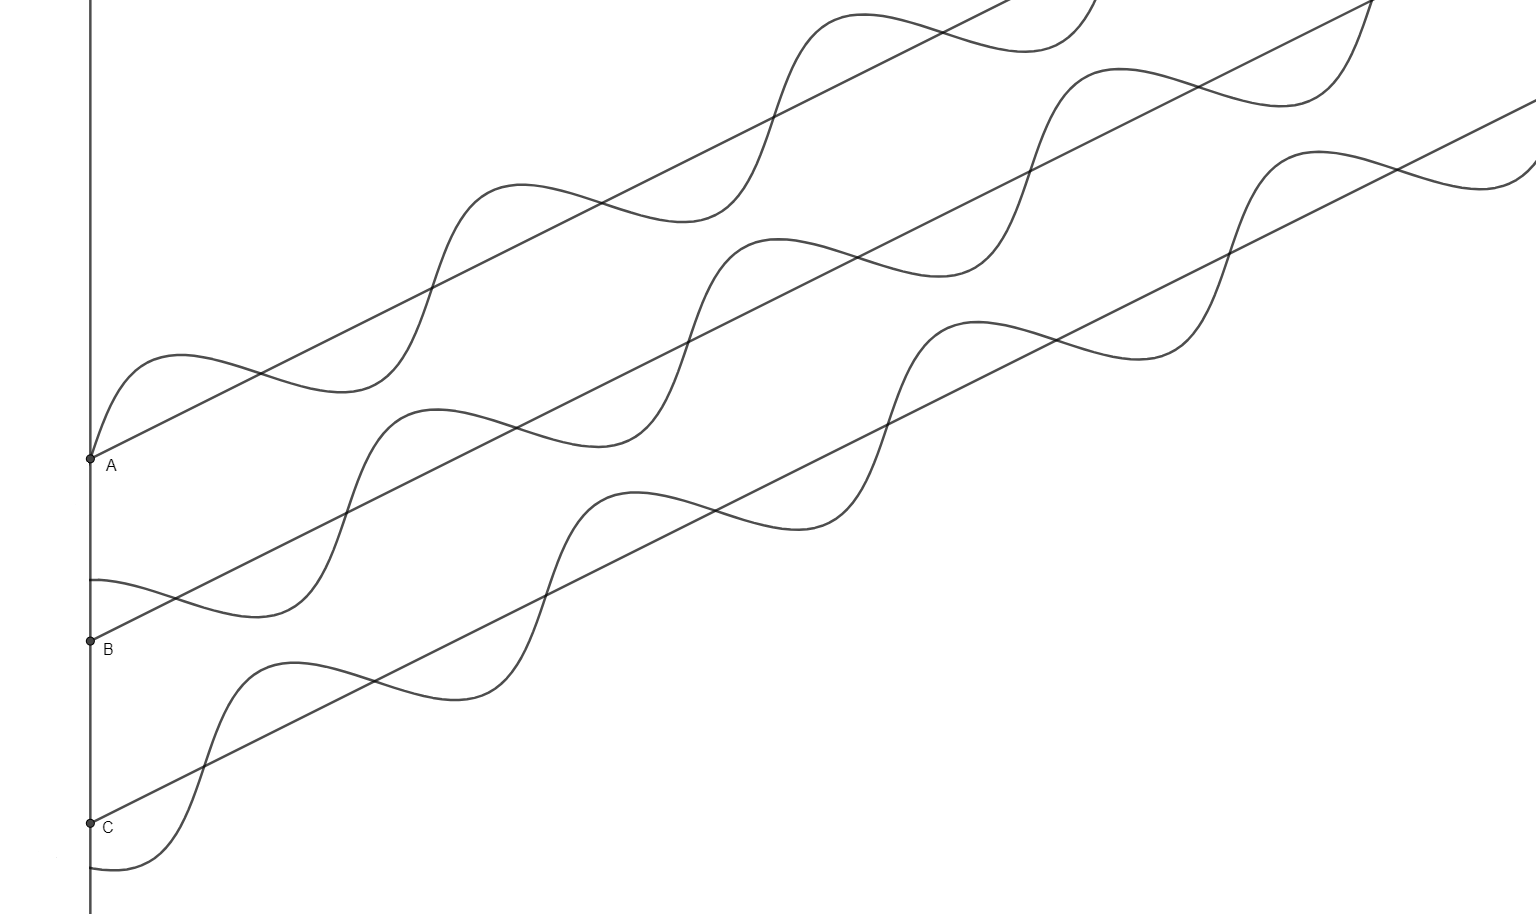
\includegraphics[width=\linewidth]{fig_uno.png}
    \caption{Rays emerging from 3 slits.}
    \label{fig:rays}
  \end{figure}
\newpage
Due to the small distance between the slits, all of the emerging rays will be close to parallel. Then by drawing a perpendicular, the following figure can be constructed:
\begin{figure}[h!]
  \centering
  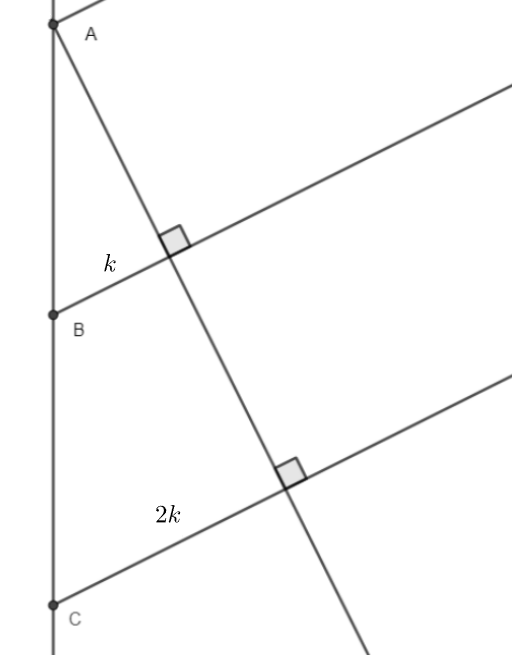
\includegraphics[scale=0.5]{figure_dos.png}
\end{figure}
\\Let the base of the smallest right-angled triangle be $k$. Since any two adjacent slits are equidistant, by property of similar triangles, the length of each subsequent base will
increase by $k$. In other words, for each subsequent slit, the \underline{phaseshift} will be increased by $k$.
\\
\\
Say that each ray has wavelength $\lambda$. By thinking of the slits as the origin, we can express each ray as a function.
Using our knowledge of sinusoids from our Grade 11 Functions course, we can express each ray as $\sin(\frac{2\pi}{\lambda}(x+jk))$, where $j$ is some integer from $0$ to $n-1$. 
For example, from the figure above, the ray that emerges from point A has a sine wave of $\sin(\frac{2\pi}{\lambda}x)$, the wave from point B is $\sin(\frac{2\pi}{\lambda}(x+k))$ and so on. 
From these expressions, we can recognize that when $k = \lambda$, all of the waves will be completely in-phase and interfere \textbf{constructively}, resulting in a light fringe being
observed on the screen. 
\newpage
In fact, if $k$ is any integer multiple of $\lambda$, there will be a light fringe.
For there to be a dark fringe, with the restriction of $0<k < \lambda$, we would like to find values of
$k$ such that the sum of the waves is zero everywhere. We are considering values of $k$ within one wavelength. We will handle values of $k$ beyond one wavelength 
when we begin deriving formulae. 
\\
\\
Using sigma notation, this sum can be expressed as:
\begin{equation}
  \label{eqn:1}
  \sum_{j=0}^{n-1} \sin(\frac{2\pi}{\lambda}(x+jk)) = 0
  \end{equation}
But since the sine and cosine graphs have the same shape, the following must also be true:
\begin{equation}
  \label{eqn:2}
  \sum_{j=0}^{n-1} \cos(\frac{2\pi}{\lambda}(x+jk)) = 0
  \end{equation}
The two sums can be combined into:
\begin{equation}
  \label{eqn:3}
  \sum_{j=0}^{n-1} \cos(\frac{2\pi}{\lambda}(x+jk)) + \sin(\frac{2\pi}{\lambda}(x+jk)) = 0
  \end{equation}
Hmmm....
\\Rather than viewing the summands purely as functions, think of vector components. Instead of $x+jk$ being mere inputs, view them as actual angles.
Then the question is the same as asking: If we have $n$ vectors all $\frac{2\pi k}{\lambda}^\circ$ apart with the first vector having angle $\frac{2\pi x}{\lambda}^\circ$,
for what values of $k$, with $0<k<\lambda$, will the sum of these vectors be 0? 
\newpage
\section{The Idea of Vector Numbers}
Complex numbers have many interesting properties. For example, when looking at the powers of $i$:
$$i$$
$$i^2 = -1$$ 
$$i^3 = -i$$
$$i^4 = 1$$
$$i^5 = i$$
$$\vdots$$
We see that the powers of $i$ repeat with period 4. 
\\

Complex numbers come in two forms: rectangular and polar. 
In rectangular form, the complex number is expressed as $z = a + bi$. It is common convention to use $z$ as a complex variable just as 
$x$ is commonly used as a real number variable. In polar form, the complex number is expressed
$z = re^{i\theta}$ or $z = r(\cos\theta + i\sin \theta)$, where $e$ is Euler's constant, $r$ is the \textbf{modulus} and $\theta$ is called the \textbf{argument}. The \textbf{argument} is the angle measured counter clockwise from the real axis 
to the complex number. Here, we will abbrviate $r(\cos\theta + i\sin \theta)$ to $r\text{c}i\text{s}\theta$. 

\newpage
Let's look at an example:
\begin{figure}[h!]
  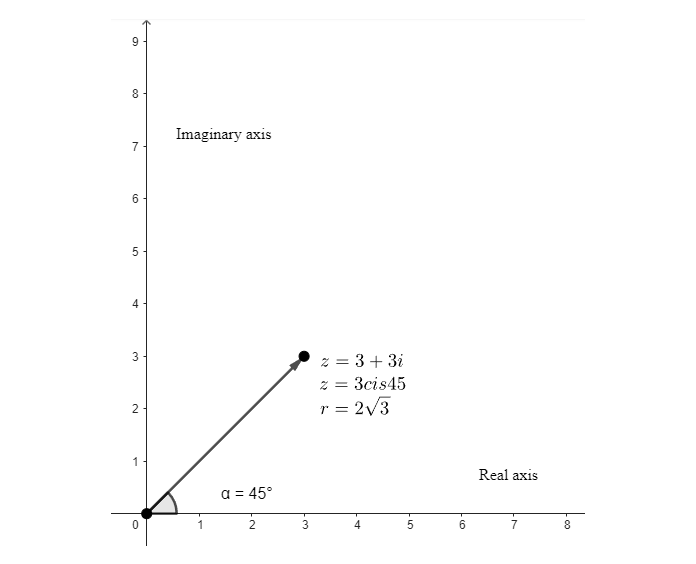
\includegraphics[width=\linewidth]{complexdiagram.png}
  
\end{figure}

Hmmm....
\\It is as if vectors are built into complex numbers. The real portion describes its position along a horizontal axis and the imaginary portion describes its position along a vertical axis.
Rather than needing to describe a vector as two coordinates or even a matrix, we can use complex numbers. As a matter of fact, complex numbers are sometimes referred to as \textbf{vector numbers}.
\\So let us change equation (3) into
\begin{equation}
  \label{eqn:4}
  \sum_{j=0}^{n-1}[\cos(\frac{2\pi}{\lambda}(x+jk)) + i\sin(\frac{2\pi}{\lambda}(x+jk))] = 0
  \end{equation}
But why might this be useful? 
\section{De Moivre's Theorem}
Consider the following complex numbers $$z_{1}=r_{1}(\cos\theta_{1}+i\sin\theta_{1})$$
$$z_{2}=r_{2}(\cos\theta_{2}+i\sin\theta_{2})$$
\\If we look at their product:
$$z_{1}z_{2}=r_{1}r_{2}(\cos\theta_{1}+i\sin\theta_{1})(\cos\theta_{2}+i\sin\theta_{2})$$
$$=r_{1}r_{2}[(\cos\theta_{1}\cos\theta_{2}-\sin\theta_{1}\sin\theta_{2})+i(\sin\theta_{1}\cos\theta_{2}+\sin\theta_{2}\cos\theta_{1})]$$
$$=r_{1}r_{2}[\cos(\theta_{1}+\theta_{2})+i\sin(\theta_{1}+\theta_{2})]$$
We find that the product of $z_{1}$ and $z_{2}$ is equivalent to rotating and scaling a complex number. How might we use this?
\\
\\
De Moivre's Theorem states that for integer $n$,
$$(r\text{c}i\text{s}(\theta))^n = r^n\text{c}i\text{s}(n\theta)$$
You can think of it as repeatedly rotating $r\text{c}i\text{s}(\theta)$ by $\theta$ and scaling it by a factor of $r$ each time.
\newpage
\section{Bringing it all together}
We are able to seperate the arguments in equation (4)
$$\sum_{j=0}^{n-1} \text{c}i\text{s}(\frac{2\pi}{\lambda}(x+jk))=0$$
$$\text{c}i\text{s}(\frac{2\pi x}{\lambda})\sum_{j=0}^{n-1}\text{c}i\text{s}(\frac{2\pi jk}{\lambda})=0$$
Using De Moivre's Theorem, since $j$ is always an integer, we can bring $j$ outside:
$$\text{c}i\text{s}(\frac{2\pi x}{\lambda})\sum_{j=0}^{n-1}\text{c}i\text{s}(\frac{2\pi k}{\lambda})^j=0$$
Then this becomes a geometric series.
\\The sum is then equivalent to: 
$$\text{c}i\text{s}(\frac{2\pi x}{\lambda})\frac{1-\text{c}i\text{s}(\frac{2\pi k}{\lambda})^n}{1-\text{c}i\text{s}(\frac{2\pi k}{\lambda})}=0$$
\begin{equation}
\text{c}i\text{s}(\frac{2\pi x}{\lambda})\frac{1-\text{c}i\text{s}(\frac{2\pi nk}{\lambda})}{1-\text{c}i\text{s}(\frac{2\pi k}{\lambda})}=0
\end{equation}
For this equation to be zero for \textbf{all} values of $x$, the numerator of the fraction must be 0.
\\Then,
$$\text{c}i\text{s}(\frac{2\pi nk}{\lambda})=1$$
$$\text{c}i\text{s}(\frac{2\pi nk}{\lambda})=\text{c}i\text{s}(2\pi t)$$
where in the above, $t$ is some integer. 
\\
\newpage
Continuing,
$$\frac{2\pi nk}{\lambda}=2\pi t$$
\begin{equation}
 k = \frac{t\lambda}{n} 
 \end{equation}

Putting the above relation into our constraints for $k$,
$$0<\frac{t\lambda}{n}<\lambda$$
$$0<t<n$$
Since $t$ is an integer, 
$$t = \{1,2,3,\ldots,n-1\}$$
From these values of $t$, we can construct a solution set for $k$:
$$k = \bigg\{\frac{\lambda}{n}, \frac{2\lambda}{n},\frac{3\lambda}{n}, \ldots, \frac{(n-1)\lambda}{n}\bigg\}$$
$\therefore$ For $n \geq 2$ slits, there exists $n-1$ darkfringes
\newpage
\section{Deriving equations}
We are now ready to derive equations that can predict where dark fringes may occur. Consider the following figure:
\begin{figure}[h!]
  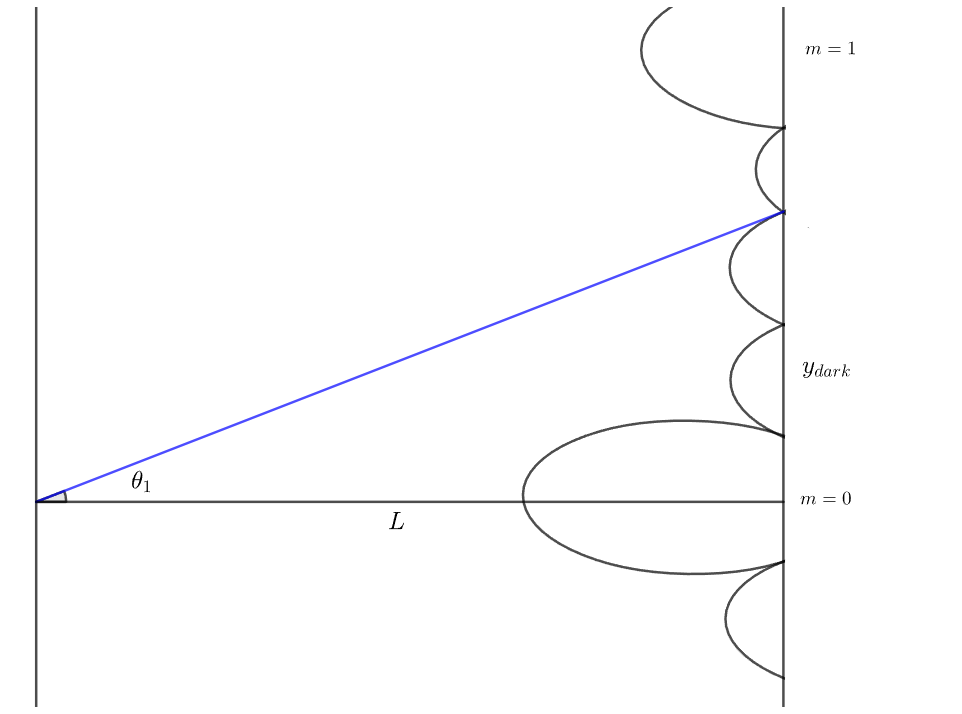
\includegraphics[width=\linewidth]{fig_three.png}
\end{figure}
\\Here in the diagram, $L$ is the horizontal distance, $y_{dark}$ is the vertical distance from the source to a dark fringe, and $m$ is the order $(m = 0,1,2, \dots)$. The order just means how many wavelengths away a point is from
the source. Although we may have multiple slits, due to the extremely small spacing between them, we consider all the slits to be one collective source. From the above diagram, we find that $\tan \theta_{1} = \frac{y_{dark}}{L}$.
\newpage
Looking at the ``top most" rays, we construct the diagram below:
\begin{figure}[h!]
  \centering
  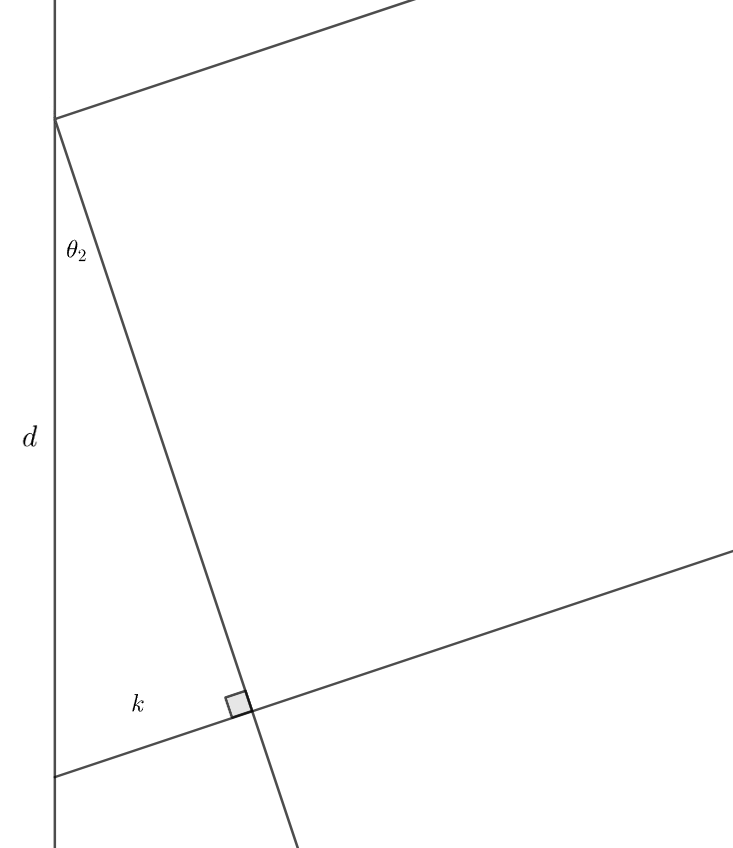
\includegraphics[scale=0.54]{simtriangle.png}

\end{figure}

Then from the figure above, $\sin \theta_2 = \frac{k}{d}$. \\But since both $\theta_1$ and $\theta_2$ are very small:
$$\tan \theta_1 \approx \sin \theta_2$$
$$\frac{y_{dark}}{L} \approx \frac{k}{d}$$
$$y_{dark} \approx \frac{kL}{d}$$
By including the order,
$$y_{dark} \approx \frac{(k+m\lambda)L}{d}$$
\newpage
But since $k$ must take on values from the solution set above, 
$$y_{dark} \approx \bigg\{\frac{\lambda L(nm+1)}{nd}, \frac{\lambda L(nm+2)}{nd},\frac{\lambda L(nm+3)}{nd}, \ldots, \frac{\lambda L(nm+n-1)}{nd}\bigg\}$$
As a sanity check, let's see if the above agrees with the equation for two slits.
\\
\\Since $n = 2$ in this case, 
$$y_{dark} \approx \frac{\lambda L(2m+1)}{2d} = \frac{(m+\frac{1}{2})\lambda L}{d}$$
which agrees with the formula found in the textbook.
\newpage
\section{Conclusion}
We were able to prove that for $n \geq 2$ slits there exists $n-1$ dark fringes and with this information,
we are able to predict where these dark fringes may occur. In this process, we have also gained some exposure on complex numbers.
This is a very niche application of complex numbers, it just so happens that we were able
to make use of De Moivre's Theorem in order to determine values of $k$. 
\\
\\
If there is one thing to take away from this, it isn't knowing about De Moivre's Theorem or 
any of the new math that you may have been exposed to. Rather, I hope that by reading this, even if you can't fully follow along, it encourages you to think more about your courses 
outside the classroom, regardless of the subject. And it does not have to be something complicated! Just the mere act of putting in a \textbf{consitent} effort to think
about your subjects will go an extremely long way. Studying for a grade is one thing but studying to get a grasp on the subject is another.
\\
\\
Learning is not something that is one sided. Our teachers can only put the components in our hands. It is up to us students,
in our own time, to put these pieces together so that we can gain a more complete understanding of the subjects that we are learning. 



\end{document}